% -*- coding: utf-8 -*-

\section{Rectangular Swept Spheres}
\label{rss}

\subsection{Introduction}
In this section I will go into greater detail about the RSS, how it is defined and represented, as well as the literature that I have used in this report. I will also shortly describe Point Swept Spheres (PSS) and Line Swept Spheres (LSS), which are similar to RSS'. No other bounding volumes will be described. 

\subsection{Rectangular Swept Sphere}
The Rectangular Swept Sphere (RSS) is a 3D figure. It is generated by taking a sphere with a positive radius and sweeping it over a rectangle in 3 dimensional space. This makes it resemble a rectangular rounded pillow. An illustration of a RSS can be found in figure \ref{rss-example-figure} on page \pageref{rss-example-figure}. 

\subsection{Representation of RSS}
I have chosen to represent the RSS as a rectangle in 3D together with a radius, as described in \cite{larsen00fast}, \cite{Larsen99fastproximity} and \cite{237244}. The rectangle is represented by 2 vectors, both of their length, a center point, and the list of points that defines it. See section \ref{rectangle3d} page \pageref{rectangle3d} for  implementation details. I felt this was best way to represent it, as it adequately described the RSS, took up a minimum of space, contains the vectors, and follows the representation found in \cite{237244}, which is useful, as I use the axis-separation test described in the article.

\begin{figure}
\centering
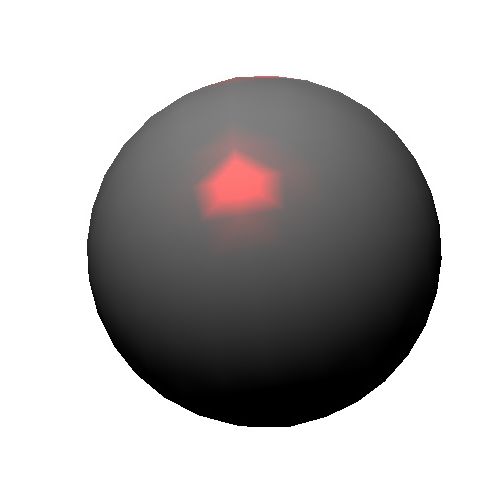
\includegraphics[width=0.5\textwidth]{figures/pss}
\caption{\label{pss-example}An example of a PSS}
\end{figure}

\subsection{Point Swept Spheres}
A point swept sphere is a BV that is created by taking a point p in 3D, and placing the center point of a sphere s with a positive radius at p. The advantage of the PSS is that it is both simple to implement and to check to for intersection with other PSS. PSS can however easily get a large volume, as the only properties that can be changed is its radius and its center point. A BVH using PSS are therefore likely to need more intersection checks than other BVs, such as LSS' (see below) or RSS'.

\begin{figure}
\centering
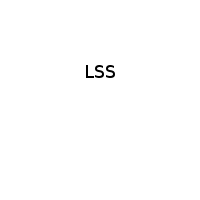
\includegraphics[width=0.5\textwidth]{figures/lss}
\caption{\label{lss-example}An example of a LSS}
\end{figure}

\subsection{Line Swept Spheres}
A line swept sphere is a BV that is created by taking a line segment l, placing the center point of a sphere s with a positive radius on one of the endpoints of l, and then sliding s to the other endpoint of l. It is a bit harder to check for intersection in LSS' than PSS' (see above), but LSS in practice have a tighter fit for the points it contains, and will therefore create fewer unneeded checks for intersection than the PSS' BV.

\begin{figure}
\centering
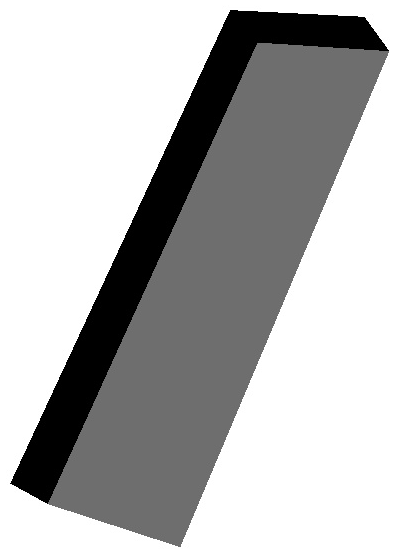
\includegraphics[width=0.5\textwidth]{figures/obb}
\caption{\label{obb-example}An example of a OBB}
\end{figure}

\subsection{OBB}
The Oriented Bounding Box is a Box of a certain positive height, width and length, and which has an orientation - i.e. is not necessarily axis-oriented. For an example of an OBB, see figure \ref{obb-example}. As I will explain later, RSS' and OBB's based on the same point set should have a similar volume - with the RSS in most cases having a volume that is slightly larger. 

\subsection{Literature used in this report}
For this project I have used the following literature:
\begin{description}
\item[\cite{larsen00fast}] Gives an introduction to some of the problems with making Distance Queries between RSSs. The article refers \cite{Larsen99fastproximity} (by the same authors) which contains more explicit information on how to calculate the distance. 
\item[\cite{Lotan03algorithmand}] Gives a general introduction to Monte Carlo simulation of Proteins, as well as a comparison of several data-structures and algorithms for these, for protein folding. None of the material in this article is used directly, but rather as background material.
\item[\cite{Larsen99fastproximity}] A more in-depth description of how the distance queries for the RSSs can be preformed. However, it leaves the most difficult cases to \cite{237244}.
\item[\cite{237244}] A description the algorithm for the most difficult case of RSS distance query. Although the algorithm as described is for Oriented Bounding Boxes (OBB).
\end{description}

\subsection{Conclusion}
I have in this section described the Rectangular Swept Sphere, as well as the 3 other BV that I that I will work with throughout this report. I have furthermore given an example of all 4 BVs, and shortly discussed the main literature..
